\documentclass{szzclass}

\title{Přehled Chomského hierarchie formálních jazyků a gramatik. Turingovy stroje. Třídy problémů P, NP, NP-těžký, NP-úplný.}
\author{Jakub Rathouský}

\begin{document}
\maketitle
\tableofcontents
\newpage

\section{Přehled Chomského hierarchie formálních ja\-zyků a gramatik}

\begin{figure}[ht]
    \centering
    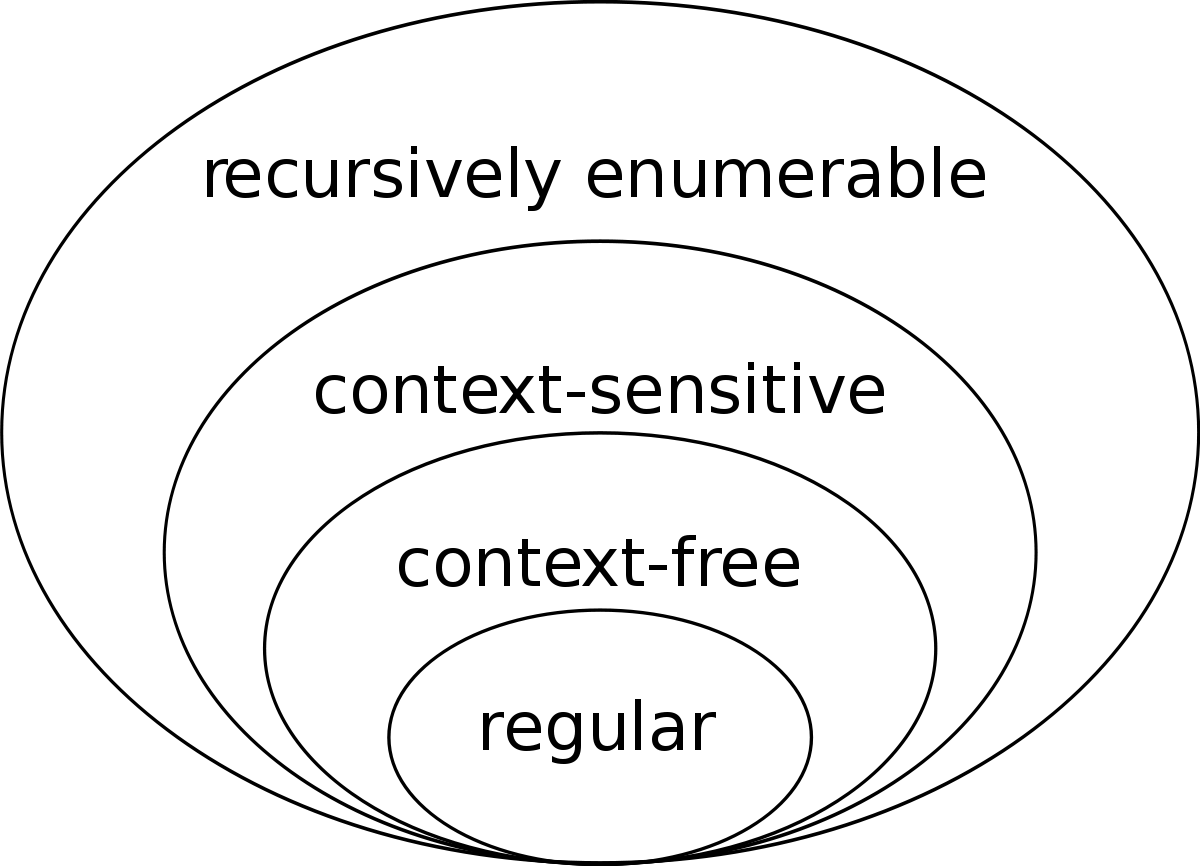
\includegraphics[width=0.6\textwidth]{topics/bi-spol-01/images/Chomsky_hierarchy.png}
    \caption{Chomského hierarchie formálních jazyků a gramatik}
\end{figure}

\begin{itemize}
\item\textit{Regulární jazyk}
vždy zároveň bezkontextový, kontextový a rekurzivně spočetný
\item\textit{Bezkontextový jazyk}
vždy kontextový a rekurzivně spočetný
\item\textit{Kontextový jazyk}
vždy rekurzivně spočetný
\end{itemize}

\subsection{Regulární jazyk}
Nejjednodušší množina formálních jazyků, formální jazyk je regulární, když lze:
\begin{itemize}
\item přijmou \textbf{(ne)deterministickým konečným automatem}
\item generovat \textbf{regulární gramatikou}
\item popsat \textbf{regulárním výrazem}
\end{itemize}

\subsection{Bezkotextový jazyk}
Formální jazyk je bezkontextový, když lze:
\begin{itemize}
\item přijmou \textbf{nedeterministickým zásobníkovým automatem}
\item generovat \textbf{bezkontextovou gramatikou}
\end{itemize}
Například výraz $A^nB^n$ není regulární, ale je kontextový a rekurzivně spočetný.

\subsection{Kontextový jazyk}
Formální jazyk je kontextový, když lze:
\begin{itemize}
\item přijmou \textbf{nedeterministickým lineárně omezeným Turingovým strojem}
\item generovat \textbf{kontextovou gramatikou}
\item generovat \textbf{nezkracující gramatikou}
\end{itemize}
Například výraz $A^nB^nC^n$ není bezkontextový ani regulární, ale je rekurzivně spočetný.

\subsection{Rekurzivně spočetný jazyk}
Formální jazyk je rekurzivně spočetný, když lze:
\begin{itemize}
\item přijmou \textbf{(ne)deterministickým Turingovým strojem}
\item generovat \textbf{neomezenou gramatikou}
\end{itemize}
Například (problém nasazení)L = {R : Turingův stroj R nepřijímá vstup R}.

\section{Turingovy stroje}
Turingův sttoj se skládá z \textbf{řídící jednotky}, \textbf{neomezené čtecí pásky} rozdělené do buněk a \textbf{čtecí hlavy}.
Čtecí hlava se umí pohybovat oběmy směry, či posečkat na stejném místě.
\newline
Formální definice Turingova stroje je:

uspořádaná \textbf{sedmice: R = (Q, $\Sigma$, G, $\delta$, $q_0$, B, F)}.
\begin{itemize}
\item Q je konečná neprázdná množina stavů
\item $\Sigma$ je konečná vstupní abeceda
\item G je konečný neprázdná pracovní abeceda ($\Sigma$ $\subset$ G)
\item $\delta$ je přechodová funkce (liší se u jednotlivých TS)
\item $q_0$ počáteční stav
\item B $\in$ (G bez $\Sigma$) je prázdný symbol (BLANK)
\item F $\leq$ Q je množina koncových stavů
\end{itemize}
Na začátku vypočtu se nachází TS v počátečním symbolu $q_0$, páska je vyplněna BLANK znaky, na "prvních" buňkách pásky je zapsán vstup a čtecí hlava ukazuje na první buňku vstupu.
\newline
Konfigurace obecně je prvek $<q,s,n>$, kde \textit{q} je aktuální stav, \textit{s} je nejmenší souvislá část pásky obsahující všechny neprázdné symboly a \textit{n} je pozice čtecí hlavy.
\subsection{Deterministický Turingův stroj}
Má následující přechodovou funkci $\delta$:

$\delta$ je zobrazení z (Q bez F) x G do Q x G x \{-1, 0, 1\}
\newline
Je-li TS v \textbf{nekoncovém} stavu a z pásky \textbf{čte} nějaký symbol z pracovní abecedy, poté \textbf{přejde} do dalšího stavu, na pásku \textbf{zapíše} nějaký symbol
a čtecí hlava se \textbf{posune}.
\newline
Je-li TS v \textbf{koncovém} stavu, \textbf{zastaví se} a dál \textbf{nepokračuje}.
\newline
\begin{itemize}
\item pro každý symbol má jasně dán přechod
\item pro špatnou kombinaci stroj skončí s chybou a vstup nepřijme
\item TS se zastaví právě tehdy, když přejde do koncového stavu
\end{itemize}

\subsection{Nedeterministický Turingův stroj}
Má následující přechodovou funkci $\delta$:

$\delta$ je zobrazení z (Q bez F) x G do množiny všech podmnožin množiny Q x G x \{-1, 0, 1\}
\newline
\newline
Na rozdíl od DTS může mít v daném stavu několik přechodů pro daný symbol.
NTS si tedy může vybrat, jakým způsovem bude ve výpočtu pokračovat.

\subsection{Porovnání síly výkonu TS}
NTS je stejně výkonný jako DTS.
\subsection{Formální zápis}
(DTS) $\delta$(S, a) = (A, c, 1) = ze stavu S na symbol a se přesune do stavu A, zapíše symbol C a posune se o 1.
\newline
(NTS) $\delta$(S, a) = \{(A, c, 1), (B, r, -1)\}
\subsection{Přijímání řetězce}
NTS \textbf{přijme} vstupní řetězec, pokud existuje aspoň jedna posloupnost přechodů, kdy TS přejde do koncového stavu a páska je na konci výpočtu prázdná.
\newline
NTS \textbf{nepřijme} vstupní řetězec, pokud každá posloupnost skončí jako u DTS.
\newline
\newline
DTS \textbf{přijme} řetězec pokud přejde do koncového stavu a páska je po skončení vyplněná prázdnými symboly BLANK.
\newline
DTS \textbf{nepřijme} řetězec pokud:
\begin{itemize}
\item dojde-li během výpočtu k chybě v podobě nedefinovaného přechodu
\item pro daný vstup neskončí (zacyklí se)
\item přejde do koncového stavu, ale páska není po ukončení výpočtu prázdná
\end{itemize}

\subsection{Lineárně omezený TS}
\begin{itemize}
\item nesmí použít neomezený počet buněk na pásce
\item na začátku výpočtu si zvolí konstantu K a daný TS se během výpočtu může pohybovat pouze na K*(délka vstupu) buňkách pásky
\end{itemize}

\subsection{Vícepáskový TS}
\begin{itemize}
\item má více pásek a více čtecích hlava
\item jednopáskové a více páskové TS jsou stejně výkonné
\end{itemize}
\subsection{Kódovanání TS}
\begin{itemize}
\item zakódování přechodové funkce TS do řetězce nad jeho abecedou
\item nekonečná paměť TS lze zakódovat do konečného řetězce
\item výsledná množina stavů je konečná, abeceda je konečná i pravidla jsou konečné
\end{itemize}
\subsection{Univerzální TS}
\begin{itemize}
\item dostane na vstupu zakódovaný TS a řetězec w
\item univerzální TS pak simuluje výpočet TS nad řetězcem w
\item$R_u$ tedy vstup přijme (nepřijme) právě tehdy, když jej příjme (nepříjme) R
\item Formální zápis: L($R_u$) = $L_n$, kde $L_n$ = \{[R,w], TS R přijmá řetězec w \}
\end{itemize}
\subsection{Rozhodování jazyka}
TS R rozhoduje jazyk L, jestli-že jej příjmá a výpočet se pro každé slovo zastaví.
\newline
Pro w$\in$L $\Rightarrow$ přejde do koncového stavu a páska \textbf{je} prázdná.
\newline
Pro w$\notin$L $\Rightarrow$ přejde do koncového stavu a páska \textbf{není} prázdná.
\newline
Tedy pro $\forall$w$\notin$L se TS \textbf{zastaví}.


\section{Třídy problémů P, NP, NP-těžký, NP-úplný}
\subsection{Rozhodovací problém}
Rozhodovací problém je takový problém, na který je odpovězeno Ano nebo Ne. Rozlišují se instance Ano-instance a Ne-instance
pro použití TS se instance namapují na \{1,0\}*. Všechny Ano-instance tvoří jazyk $L_a$. TS řeší rozhodovací problém, pokud rozhodne $L_a$.
\subsection{Optimalizační problém}
Optimalizační problém je problém, který hledá v nějakém ohledu optimální řešení. Pro lepší názornost se používá rozhodovací verze problému.
Optimalizační a rozhodovací verze jsou výpočetně stejně náročné.
\subsection{Rozhodnutelné problémy}
(Ne)Rozhodnutelné problémy jsou problémy, pro které existuje algoritmus, který je řeší. Nerozhodnutelný problém je ten, který není rozhodnutelný.
\newline
Rozhodnutelný problém odpovídá rekurzivnímu jazyku.
\newline
Nerozhodnutelný problém odpovídá nerekurzivním jazykům.
\subsection{Třída P}
Třída rozhodovacích problémů, které lze řešit v polynomiálně omezeném čase deterministickým Turingovým strojem.
\subsection{Třída NP}
Třída rozhodovacích problémů, které lze řešit v polynomiálně omezeném čase na nedeterministickým Turingovým stroji.
Všechny P problémy patří do NP.
\subsection{Třída NP-těžký}
Problém, na který lze převést všechny problémy ze třídy NP. Sám NP-těžký problém nemusí patřit do třídy NP.
Jeden takový problém lze převést na jiný pomocí polynomiální redukce.
\subsection{NP-úplný}
Je NP-těžký a patří do skupiny NP. Jsou to nejtěžší problémy ze třídy NP. Využívají se v kryptografii.
\newline
Pokud by byl nalezen polynomiálně deterministický algoritmus pro libovolnou NP-Úplnou úlohu, všechny NP problémy by byly řešitelné.
\subsection{Polynomiální redukce}
$\leq_p$: proces který převádí problém A$\rightarrow$B (A$\leq_p$B). Dostane na vstup instanci problému A ($I_A$) a jako výstup vrátí v polynomiálním čase instanci problému B ($I_B$)
se stejnou pravdivostní hodnotou. Je-li splněno $I_A$ pak je i $I_B$.
\end{document}